\section{Persistent Storage for Mutable Variables}\label{concepts:pstore}

Section \ref{concepts:closures} explains the process of obtaining compiled
closures. The instructions and the constant variable bindings in a compiled
closure are contained in the SECpack given to the TEM when the closure must be
executed. The overhead of decoding the same instructions and constants is much
smaller than the cost of persistent state. On the other hand, the values of the
mutable variables must persist in the TEM across closure executions. To
prevent integrity attacks that use stale data, the TEM owner cannot be trusted
with the values of mutable variables, even if the values are encrypted and
signed.

\begin{figure}[hbtp]
	\center{
		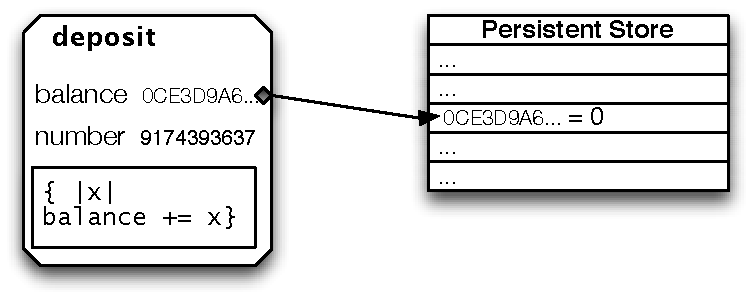
\includegraphics{omnifigs/persistent_store}
	}
	\caption{Closure with Mutable Variable Referencing the Persistent Store}
	\label{fig:persistent_store}
\end{figure}

The values of mutable variables are stored inside a secured global persistent
store (Figure \ref{fig:persistent_store}), indexed by addresses which are
guaranteed to be at least as large as a cryptographic hash. An address
identifies a value and is also proof that a closure is authorized to access
that value. The information in the persistent store is stored in a
way that prevents any accesses that would bypass the associative memory
abstraction. The implications of the requirement above are discussed in section
\ref{arch:pstore}. The following theorem proofs the security of this design.

\begin{theorem*}
Gaining unauthorized access to the value of a mutable variable is as hard as
directly breaking chain of trust.
\end{theorem*}
\begin{proof}
Gaining access to a variable is equivalent to obtaining the variable's address,
because the associative memory abstraction cannot be bypassed. Assume that the
variable's address is stored in $\mathcal P$ in the secured version of the TEM.
This holds for any well-designed secure closure. The analysis in section
\ref{concepts:secpack_binding} shows that information in $\mathcal P$ is not
leaked by repeated attempts to execute a closure, so the only possibility of
obtaining the variable's address is by guessing it.

If Mii has an oracle\footnote{non-deterministic Turing machine} that can
produce enough bits to allow Mii to guess a variable's address, then he can use
the oracle to build a false Endorsement Certificate, as follows. Mii can
generate an asymmetric key, and build a certificate for it by copying all the
other fields from the Endorsement Certificate of his TEM. Then Mii can use the
oracle to guess a value $v$ that can be assigned to one of the inessential
certificate fields (serial number, subject name, an optional field), so that
the certificate's cryptographic hash matches the new data. The essential fact
here is that an address has at least as many bits as a cryptographic hash, so
$v$ would be long enough to impact all the bits in the certificate's hash. 

Once Mii has an Endorsement Certificate for his personal key, he can convince
Yu to encrypt her secrets with his public key, thus the chain of trust is
broken. Therefore, the effort needed to gain access to the value
of a mutable variable is sufficient to break the TEM chain of trust directly.
\end{proof}

Section \ref{concepts:pstore_auth} shows that the use of addresses as
authorization values is robust and does not raise any issues when the closure
is put together. The persistent store design presented here is minimal, as
demonstrated in section \ref{concepts:pstore_minimal}. Chapter
\ref{arch} demonstrates the practicality of these concepts, by presenting an
architecture built on top of them.

\subsection{(No) Considerations for Authorizations}\label{concepts:pstore_auth}

The use of value addresses as authorization values may concern
software developers, because intuition dictates that, under this design,
closures should not use too many variables, to minimize the surface area
for a guessing attack. The result below dissipates this concern, by showing
that closures using a high number of variables are as safe as closures using
one variable. The theorem presented here can also be used to conclude that it is
safe for a closure to use consecutive persistent store addresses.

\begin{lemma*}
Compromising a closure using $N$ mutable variables is equally hard if the
authorization secrets are randomly distributed or consecutive numbers.
Furthermore, either closure is insignificantly easier to compromise than a
closure with a single mutable variable.
\end{lemma*}
\begin{proof}
Let $b$ be the size of the authorization secrets, in bits. Then
$\mathcal U = 2^b$ is the size of the universe of authorization secrets.
Section \ref{concepts:secpack_binding} shows that no information on
authorization secrets is leaked as long as they are correctly classified as
private (in $\mathcal P$), so the only attack on mutable variables is guessing
values directly.

It follows that attacks on mutable variables are (educated) guesses of their
authorization values. Assuming an attacker makes perfect use of his knowledge
of address distribution, and stops upon a successful guess, the guesses can be
considered independent probes. So the probability of success after $g$ guesses
is $p_g = 1 - (1 - p_1)^g$, where $p_1$ is the probability that a single
guess will be successful.

The probability that a random guess matches one of the $N$
authorization secrets is $\frac{N}{\mathcal U}$, regardless of the
distribution of the $N$ variables. An attacker with full information on the
distribution of the secrets can improve his chances of success to
$p_1 = \frac{N^2}{\mathcal U}$, in the best case (e.g., if the secrets are
consecutive, the attacker would probe one out of every $N$ addresses).

The number of guesses $g(\alpha, N)$ required to compromise one of the $N$
variables with probability $g(\alpha, N)$ is given by the equation:
$$ 1 - (1 - \frac{N^2}{\mathcal U})^{g(\alpha, N)} = \alpha $$
which solves to: $$g(\alpha, N) = \frac{\log(1 - \alpha)}{\log(1 -
\frac{N^2}{\mathcal U})}$$

For the lack of a better definition, assert that the number of variables
$N$ has no impact on security if it causes the loss of less than one bit of
security. In other words, the number of bits that the attacker needs to guess
is reduced by one. This is equivalent to $g(\alpha, N) = 2g(\alpha, 1)$, which
resolves to:
$$
\begin{array}{rcl}
\log\Big(1 - \frac{N^2}{\mathcal U}\Big) &=& \frac{1}{2}\log\Big(1 -
\frac{1}{\mathcal U}\Big)
\\
1 - 2\frac{N^2}{\mathcal U} + \frac{N^4}{{\mathcal U}^2} &=& 1 -
\frac{1}{\mathcal U}\\
N^4\big(\frac{1}{\mathcal U} \cdot \frac{1}{\mathcal U}
\big) - 2N^2\frac{1}{\mathcal U} &=& \frac{1}{\mathcal U} \\
N^4 - N^2\cdot 2\mathcal U - \mathcal{U} &=& 0\\
N &=& \sqrt{\mathcal U - \sqrt{\mathcal{U}^2 - \mathcal U}} \\
&=& \sqrt{\sqrt{\mathcal U}(\sqrt{\mathcal U} - \sqrt{\mathcal U - 1})}
\end{array}
$$
Using the easy to prove fact that $\sqrt{x} - \sqrt{x - 1} > \sqrt[4]{x}$ for
$x \ge 4$, we obtain:
$$
\begin{array}{rcl}
\sqrt{\sqrt{\mathcal U}(\sqrt{\mathcal U} - \sqrt{\mathcal U - 1})} & > & \sqrt{\sqrt{\mathcal
 U}\sqrt[4]{\mathcal U}} \\
 & > & (\mathcal{U}^{\frac{1}{2}}\mathcal{U}^{\frac{3}{4}})^{\frac{1}{2}} \\
 & > & \mathcal{U}^{\frac{3}{8}} \\
 & > & 2^{\frac{3}{8}b} 
\end{array}
$$

So the number of variables $N$ has no impact on security as long as $N \le
2^{\frac{3}{8}b}$. In practice, authorization secrets will be at least 128-bit
long, so closures can use as many as $2^{48} \approx 2.81 \times 10^{14} $
variables.

The memory inside a TEM will burn out before these many variables are ever
used. Using a variable implies writing to it at least once, and a persistent
store write shall cause a change of at least 1 byte inside the TEM's
memory\footnote{The TEM needs to acknowledge the change, so it can ensure
freshness.}. Thus, $2^{48}$ writes will completely wear out every byte in a 2GB
EEPROM with a lifetime of 100,000 writes per byte, even assuming
perfect memory utilization. Today's high-end secure chips have approximately 100KB of
secure non-volatile memory.

In conclusion, for all practical purposes, developers are free to use as many
variables as needed, as well as any method for allocating addresses that is
convenient and doesn't introduce security holes by itself. Section
\ref{arch:ps_alloc} describes an approach for allocating addresses that is
suitable for the TEM.
\end{proof}

\subsection{Minimality of the Persistent Store
Design}\label{concepts:pstore_minimal}
This section argues for the minimality of the design discussed above. Given the
desire that the TEM be implemented in low-cost hardware, minimality of design is
very important. The presentation begins with a lemma, then continues with the
main proof that relies on the lemma.


\begin{lemma*}
If trusted execution is required, integrity must be guaranteed for all the
values of mutable variables.
\end{lemma*}
\begin{proof}
If the value of a variable does not require integrity, it can be
modified by Mii at any time. Therefore, the variable should be a parameter
supplied by Mii when the closure is executed. Assuming the closure
was designed properly, this situation would never happen, because it would
result in waste of TEM resources (persistent store entries are more expensive
than closure parameters).
\end{proof}

\begin{theorem*}
The TEM's persistent store is minimal with respect to the requirement of
trusted execution.
\end{theorem*}
\begin{proof}
Mutable variables require integrity, as proven in the lemma above. Multiple
closures may be authorized to access a variable, so the most economical
mechanism of proving authorization consists of secret values inside the
closures.

Secrets must be resistant to random guessing, so they have to be at
least as long as a symmetric encryption key. The TEM does not rely on symmetric
cryptography, so secrets must be at least as long as a cryptographic
hash\footnote{This distinction is important in practice. The standard
symmetric encryption algorithm is AES \cite{daemen1999apr}, and has 128-bit
keys, while the minimum standard for cryptographic hashes SHA1
\cite{eastlake2001rus} which produces 160-bit hashes. }, so that these secrets
do not become the weak point (easiest secrets to guess) in the TEM design. 

The need for authorized access dictates that values must have associated
authorization values with them (groups of variables can be given consecutive
addresses as shown in section \ref{concepts:pstore_auth}), so values must have
at least the same amount of data as a cryptographic hash associated with them.

Values must also be associated with unique addresses, so they can be referenced
by the binding tables of the closures using them. A minimal design will use a
single piece of data to satisfy both requirements, so it will end up using a
subset of the authorization secret as a variable's address.

Using a strict subset of the entire authorization secret as an address imposes
an uniqueness constraint over that subset, which can require special considerations
in choosing an authorization secret, as well as a supplemental security
analysis. Conversely, using the entire secret for addressing is bound to
produce a simpler design.
\end{proof}

\subsection{Read-Only Access to Mutable Variables}
The TEM's persistent store has a single authorization level -- if a closure
knows a variable's name, it has full (read/write) access to it. However,
developers may desire to offer read-only access to some mutable variables (e.g.,
a bank account's balance). This section explains two methods for implementing
read-only variables, by leveraging the TEM's design.

The TEM's owner can be allowed read-only access by offering a \textit{getter}
closure for the variable. The \texttt{balance} closure in the bank account
example in section \ref{concepts:closures} is an example of such a getter.

Read-only access can be granted to another closure by mirroring. The
contents of the variable to be acessed $v$ is duplicated in another variable
$v_R$. Every closure that changes $v$ must also change $v_R$. The address of
$v_R$ is shared with the closure that should receive read-only access. The
receiving closure is free to change the contents of $v_R$, but these changes
will not compromise the closure using $v$. Section \ref{concepts:pstore_auth}
shows that introducing the mirror variable does not have a significant impact
on the security of either variable.

